\documentclass[12pt,a4paper]{report}

\usepackage[utf8]{inputenc}
\usepackage[english]{babel}
\usepackage{amsmath}
\usepackage{amsfonts}
\usepackage{amssymb}
\usepackage{graphicx}
\usepackage{listings}
\usepackage[left=3cm,right=3cm,top=3cm,bottom=3cm]{geometry}
\usepackage{url} % formattazione url
\usepackage{color}

%colori
\definecolor{lgrey}{rgb}{0.95,0.95,0.95}
\definecolor{dblue}{rgb}{0,0,0.545}


\lstset{
	%language=c++,
	backgroundcolor=\color{white},
	basicstyle=\ttfamily\small,
	%keywordstyle=\color{dblue}\bfseries,
	%commentstyle=\color{cyan}\itshape,
	frame=tb,
	columns=fullflexible,
	showstringspaces=false,
	breaklines=true
}


% Info
\author{A. Sanfratello, A. Beconcini, F. Mola}
\title{Transformation from cartesian coordinates to polar coordinates using CORDIC}

\newcommand{\HRule}{\rule{\linewidth}{0.5mm}}

\begin{document}


\begin{titlepage}
\begin{center}
	
\includegraphics[scale=.60]{img/Unipi_logo.jpg}\\[3cm]
	\textsc{\Large Digital System Design}
	\HRule \\[0.4cm]
{ \huge \bfseries Transformation from cartesian coordinates to polar coordinates using CORDIC \\[0.4cm] }
	\HRule \\[4cm]
	\noindent
	\begin{minipage}{0.4\textwidth}
	\begin{flushleft} \large
	\emph{Authors:}\\
	Alessio Sanfratello\\
	Andrea Beconcini\\
	Francesco Mola 
	\end{flushleft}
	\end{minipage}%
	\begin{minipage}{0.4\textwidth}
	\begin{flushright} \large
	\emph{Supervisor:} \\
	Prof. Luca Fanucci
	\end{flushright}
	\end{minipage}

	\vfill
	{\large Academic Year 2014/2015}
\end{center}
\end{titlepage}

\tableofcontents


\chapter{Introduction}

\section{The CORDIC algorithm}
\label{sec:cordic_alghorithm}
The goal of this project is to design an integrated digital circuit which implements a converter from cartesian coordinates to polar ones, using the CORDIC algorithm.

CORDIC is an acronym for \emph{COordinate Rotation DIgital Computer} and it was first described by Jack E. Volder in 1959.

CORDIC has two mode of operation: \emph{rotation} and \emph{vector}. The former mode takes the coordinates of an input vector plus an angle of rotation and returns the new coordinates after the rotation has been applied.

The vector mode can convert an input vector from cartesian to polar coordinates and its result depends on multiple iterations of the CORDIC rotation mode. Basically, vector mode rotates the input vector until its \emph{y} coordinate became 0, so the modulus of the given vector is exactly equal to the value of the \emph{x} coordinate of the rotated vector and its angle is equal to the opposite of the total rotation angle.\newline
The rotation angle performed at $i$-th iteration $\alpha$ is

\begin{equation}
\alpha_{i} = \arctan \left(\dfrac{1}{2^i}\right)
\end{equation}

The reason for choosing such angles is that the rotated coordinates $x_{i+1}$ $y_{i+1}$  after $i$ rotation became

\begin{equation}
x_{i+1} = x_{i} - d_{i} y_{i}  2^{-i}
\end{equation}

\begin{equation}
y_{i+1} = y_{i} + d_{i} x_{i} 2^{-i}
\end{equation}

Where $d_{i}$ is equal to $+1$ if $y_{i} < 0$ and $-1$ otherwise.

The rotated coordinates can be computed using just sums and shift operation, as we can see in the previous equations.

The rotation performed at each stage $i$ is equal to $\alpha_{i}$ and the total rotation is given by the sum of the previous contribution such that the total rotation performed at iteration $i+1$ is

\begin{equation}
z_{i+1} = z_{i} + d_{i} \arctan \left(\dfrac{1}{2^i}\right)
\end{equation}

The results of the $\arctan()$ function can be stored in a ROM since this algorithm has to apply this function to a limited set of value. Such set depends on the number of iteration we are interested in.

Note that the CORDIC algorithm do not produce a correct output if input is equal to the null vector. In fact such input generates a null vector at every iteration while the total rotation angle keeps increasing. Such a behavior produces a wrong output.

The aim of this work is to produce a component which implements the CORDIC vector mode.

\section{Specification of requirements}

\begin{center}
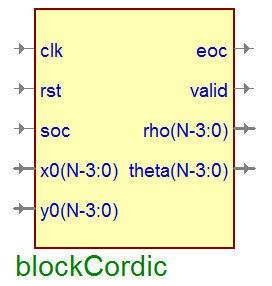
\includegraphics[scale=.50]{img/cd.jpg}\\
\end{center}
Our network has five inputs and four outputs. \emph{x0} and \emph{y0} are the Cartesian coordinates which have to be transformed in polar coordinates. 

After entering the values of these inputs the user has to put \emph{soc} to the high value (\emph{1}) to let the network starting the conversion. To obtain the result the user has to put again the input \emph{soc} to the low value (\emph{0}); when the output \emph{eoc} goes to the high value the result can be read as modulus and angle respectively in the outputs \emph{rho} and \emph{theta}, the values obtained are given in fixed point with a notation Q8.24 (8 bits for the integer part, 24 bits for the decimal part). 

The value of the angle $\theta$ is always correct and is given in radians, instead the value of the modulus $\rho$ is correct if and  only if the output \emph{valid} is on the high value, otherwise it means that the value can't be represented on two's complement on the given number of bits. 

The input \emph{rst} is low triggered.


\chapter{Architecture}

\section{Input and output notation}
Our circuit deals with 32-bit inputs and outputs in Q8.24 fixed point notation. This means our network uses 8 bits for the integer part and 24 bits for the decimal part of its input and output data.

This notation let us represent value in the interval $ \left[ -128; 127.9999999 \right]$ and it gives us enough precision to represent $2^{-24}$ radians.

\section{ROM and addresses generator}
In order to compute the rotation angle at each iteration, we need the value of $\alpha_{i}$ for each possible iteration $i$.

As we said in section \ref{sec:cordic_alghorithm}, we use a 64x32bit ROM to store the arctan() values.

The ROM is filled such that the first 25 location contain angles $\alpha$ like

\begin{equation}
\alpha_{i} = \arctan \left( - \dfrac{1}{2^{i}} \right) \mbox{ with} \; i \in \left[0; 24 \right]
\end{equation}

The location from address 32 to 56 are filled with angles $\alpha$ like

\begin{equation}
\alpha_{i} = \arctan \left(\dfrac{1}{2^{i}} \right) \mbox{ with} \; i \in \left[0; 24 \right]
\end{equation}

We can not go any further storing the arctan() values because we do not have enough precision to represent them. We choose to fill the remaining locations with zeros. Doing this, we do not modify the value of the output angle when the conversion is complete.

\section{Extender and is\textunderscore valid components}
\begin{center}
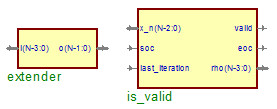
\includegraphics{img/isvalid.jpg}
\end{center}

As we discussed before, our data representation puts some limits on the range of signals we can manage. In particular there are some possible input values whose polar transformation can not be represented with Q8.24 notation.

In order to be sure whether an output is congruent with the input or not, we implement a valid mechanism.
Such mechanism takes advantages of 2 main components: \emph{Extender} and \emph{Is\textunderscore valid}.
The cordic algorithm returns the modulus multiplied by a factor of $A_{n}\sqrt{2}$ where 
\begin{equation}
A_n = \prod_{i = 0}^n{\sqrt{1+2^{-2i}}}
\end{equation}
so, $A_n$ is constant with the number of iteration we perform. The only thing we have to do to provide the modulus is to divide it by $A_n$.
When an input is provided to our network, we extend it with 2 bits more. Such extension takes into account the multiplication factor $A_n$ and we have no representation problem.

Once we have computed the result, we use the \emph{Is\textunderscore valid} to reset the validity bit if the output is not representable.

The \emph{Is\textunderscore valid} is also in charge of managing the correct sequence of control bits to drive our network. It reports the fact that the computation is over by setting the \emph{eoc} bit. Anyway the handshake protocol requires the \emph{soc} bit to be reset before setting \emph{eoc}.

\section{Counter}
Since our circuit performs multiple iterations to reach the expected output values, we need a counter to stop the computation.
We can stop the algorithm at the 25th iteration since our data format does not support precision provided with longer computation, in other words, the rotation angles after the 25th iteration are too small to be represented with Q8.24.

\section{Soc, Eoc, Rst}
We provide the user some bits to control the working status of our cordic circuit. In particular, we provide the following:
\begin{itemize}
	\item Soc (Start Of Conversion): This tells the circuit to take datas from the input bus ($x_{0}$ and $y_0$) and start the conversion.
	\item Eoc (End Of Conversion): this is an output bit set by the cordic circuit when the conversion is over and the user can read the result on the output bus (rho and theta);
	\item Rst (ReSeT): this input bit is low triggered and it must be set to 0 when we want to ensure cordic circuit to be in a consistent state, so it must be set to 0 every time the user want to perform the first conversion.
\end{itemize}

In order to drive the circuit correctly, the user must firstly set \emph{rst} to 0. Then, when the \emph{rst} is set to 1 again, \emph{soc} must assume 1 to notify the circuit that data on $x_0$ and $y_0$ are valid and the conversion can start.

\section{Starter}
Our circuit includes a specific submodule, called \emph{Starter}, in order to implement the correct starting process. The \emph{Starter} module checks the value of \emph{soc} and \emph{rst}, and it provides a reset signal to all internal registers. In particular it triggers a reset when:

\begin{itemize}
	\item \emph{rst} goes to 0;
	\item \emph{soc} goes to 1 (in this case it is kept to 0 for just 10 ns).
\end{itemize}


\pagebreak
\begin{figure}
\centering
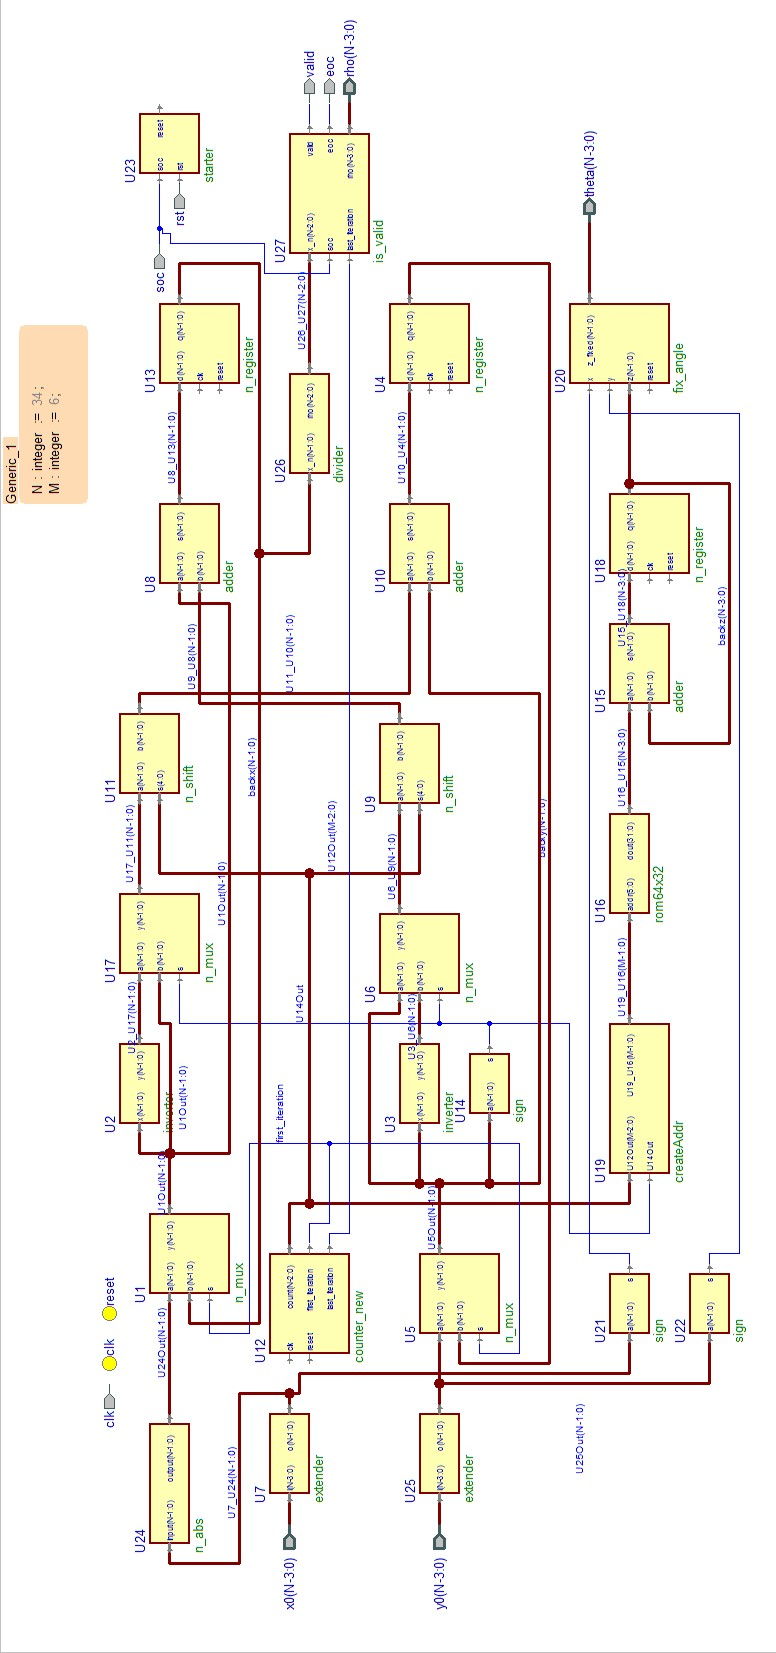
\includegraphics[scale=0.52]{img/blockCordic.jpg}
\caption{General Overview\label{fig:block}}
\end{figure}


\chapter{Testing}

\section{Design of testbench}
We designed two different kind of tests to check the correctness of both outputs rho and theta respectively.
The former ensure the modulus and validity bit while the latter validates the output angle.\\
To perform those we used a VHDL testbench file which can take an external input file containing input and expected values and compare cordic results with the expected ones.\\
The VHDL testbench and code for generating its input files can be found at section \ref{sec:test_generator}

\begin{lstlisting}[caption={A snippet from the testbench network}]
begin
	file_open(file_TEST, "test_cordic.txt", read_mode);
	rst <= '1';
	
	while not endfile(file_TEST) loop
		readline(file_TEST, v_ILINE);
		hread(v_ILINE, v_x0);	--reading first input
		hread(v_ILINE, v_y0);	--read second input
		hread(v_ILINE, v_theta);--reading expected theta
		hread(v_ILINE, v_rho);	--reading expected rho
		read(v_ILINE, v_valid);	--reading valid bit
		
		x0 <= v_x0;
		y0 <= v_y0;
		
		wait for 10 ns;
		soc <= '1' after 0 ns, '0' after 10 ns;
		wait for 10 ns;
		 
		while eoc = '0' loop
			wait for 10 ns;
		end loop;
		
		wait for 10 ns;
		
		write(v_OLINE, "rho ");
		hwrite(v_OLINE, rho);
		write(v_OLINE, " ");
		hwrite(v_OLINE, v_rho);
		write(v_OLINE, "  theta");
		write(v_OLINE, " ");
		hwrite(v_OLINE, zn);	   
		write(v_OLINE, " ");
		hwrite(v_OLINE, v_theta);
		write(v_OLINE, "  valid bit ");
		write(v_OLINE, valid);
		writeline(OUTPUT, v_OLINE);
		
		h_rho := rho(N-1 downto 16);
		h_theta := zn(N-1 downto 16);
		
		assert valid = v_valid
			report "Error on valid bit"
			severity ERROR;	  
			
		if v_valid = '1' then 
			assert h_rho = v_rho(N-1 downto 16)
				report "Error on rho"
				severity ERROR;
		end if;
			
		assert h_theta  = v_theta(N-1 downto 16)
			report "Error on theta"
			severity ERROR;	  
			
	end loop;
	
	file_close(file_TEST);
	write(v_OLINE,"End of test");	
	writeline(OUTPUT,v_OLINE);
	
	wait;
end process;
\end{lstlisting}

\subsection{Testing modulus and validity bit}
In this test we feed our circuit with coordinates of points which belongs to the function
	\begin{equation}
		y = x
  	\end{equation}
We start from point $P = \left(-127, -127\right)$ and move toward the first quadrant with a step equal to 1 until we reach point $P=(127,127)$.

Then we concentrate our tests near the point which produce a \emph{rho} overflow. Such overflow occurs around $P=(90.5,90.5)$, so we concentrate our test around that point with a step equal to 0.01 and 0.001.

\subsection{Testing angle}
After having tested the modulus output (\emph{rho}), we check the output angle correctness. We start from a point whose polar coordinates are $\rho=127$ and $\theta=0$, then we move on a circumference with an angular step equal to $\frac{\pi}{24}$.

\section{Waveform Examples}
In the following figures you can see some examples of how signals evolve in time for a couple of different inputs.

In particular in figure \ref{fig:bisector} we pass $[1,1]$ as input and after 25 iterations we obtain congruent result.


\begin{figure}[!h]
\centering
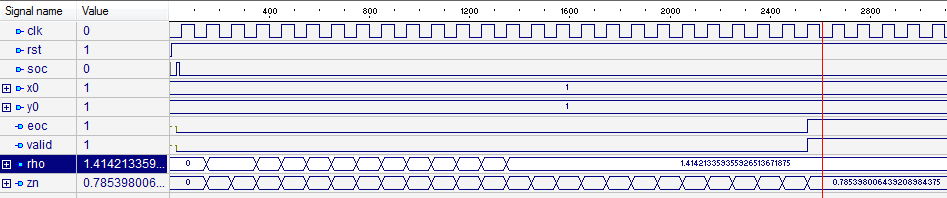
\includegraphics[width=\textwidth]{img/test-bisettrice.png}
\caption{Waveform example of valid output\label{fig:bisector}}
\end{figure}

If instead we use $[120,126]$ as input, we obtain an invalid result, therefore valid flag has been set to 0.

\begin{figure}[!h]
\centering
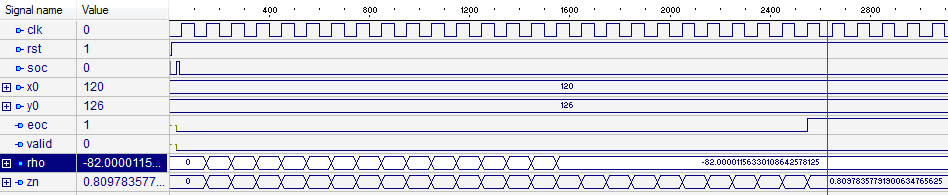
\includegraphics[width=\textwidth]{img/test-valid.png}
\caption{Waveform example of invalid output\label{fig:invalid}}
\end{figure}


\chapter{Synthesis using Xilinx ISE Tool}
At the end we decide to synthesize our project using the Xilinx ISE Tool. We decide to set a balanced design goal which automatically sets the right process properties to achieve this optimization. After that we start our synthesis.
After fixing some warnings not shown by the simulation tool, we get its result shown in the Device Utilization Summary (see figure \ref{fig:dev_utilization_summ}). 

\begin{figure}[!h]
	\centering
	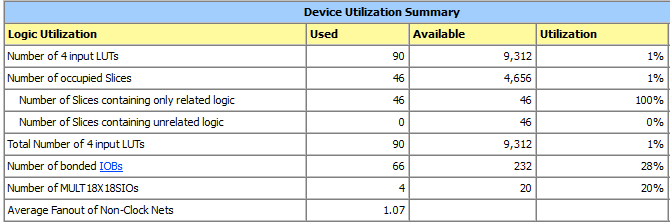
\includegraphics[scale=0.9]{img/utilizationSummary.png}
	\caption{Utilization Summary provided by Xilinx tool\label{fig:dev_utilization_summ}}
\end{figure}


In figure \ref{fig:timing_report} we can see the timing report with the calculation of the maximum path delay which gives us the relative time constraint that we have to respect in order to obtain the maximum possible frequency to drive our network.

\begin{figure}[!h]
	\centering
	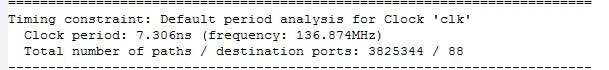
\includegraphics[scale=0.9]{img/timingReport.png}
	\caption{Timing report provided by Xilinx tool\label{fig:timing_report}}
\end{figure}


\appendix

\chapter{Source code}

\section{Generation of test data using C++}
\label{sec:test_generator}

\begin{lstlisting}[caption={Test-data generation}]
#include <stdio.h>
#include <math.h>
#include <stdint.h>

#define TWO_TO_31 0x80000000
#define MUL 16777216
#define N_ENTRIES 32
#define DIV 24

struct Polar {
    int32_t rho;
    int32_t theta;
    bool valid;
};

int32_t rom[2*N_ENTRIES];

Polar cordic(int32_t x0, int32_t y0) {
    int64_t x = 0, y = 0;
    int32_t z = 0;
    
    // Extension to "34" bits (using int64_t)
    x = x0; y = y0;
    
    // Moving to first or fourth quadrant
    x = (x < 0) ? -x : x;
    
    for (int i=0; i<=25; i++) {
        int64_t x_old = x, y_old = y;
        int32_t z_old = z;
        
        // Computing d
        int d = (y < 0) ? 1 : -1;
        
        // Computing (inverter + mux + n_shift + adder)
        x = x_old - ((d * y_old) >> i);
        y = y_old + ((d * x_old) >> i);
        
        // reading  ROM entry
        int entry = (d > 0) ? i + N_ENTRIES : i;
        
        // Computing z using ROM's value
        z = z_old + rom[entry];
    }
    
    Polar result = {0,0,false}; // Preparing result
    
    // Computing rho
    const int32_t A_n_inverted = 0x009B74ED;
    int64_t temp_rho = ((x >> 2) * A_n_inverted) >> 22;
    result.valid = (temp_rho >= TWO_TO_31) ? false : true;
    result.rho = (int32_t) temp_rho;
    
    // Computing theta
    const int32_t PI = 0x03243F6B;
    if (x0 < 0) {
        if (y0 >= 0) {
            result.theta = z + PI;
        } else {
            result.theta = z - PI;
        }
    } else {
        result.theta = -z;
    }
    
    return result;
}

void gen_rom() {
    // Computing negative values for atan(2^-i)
    for (int i = 0; i < N_ENTRIES; i++) {
        double a = (-1)*atan(pow(0.5, (double) i));
        rom[i] = (i < 25) ? (int32_t) (round(a*MUL)) : 0;
    }
    
    // Computing positive values for atan(2^-i)
    for (int i = 0; i < N_ENTRIES; i++) {
        double a = atan(pow(0.5, (double) i));
        rom[i+N_ENTRIES] = (int32_t) (round(a*MUL));
    }
}

int main() {
    gen_rom(); // Filling ROM entries
    
    // Bisector test [-127,127]
    for (int k=-127; k<=127; k++) {
        Polar p = cordic(k<<24,k<<24);
        printf("%08X %08X %08X %08X %d\n", k<<24, k<<24, p.theta, p.rho, p.valid);
    }
    
    // Bisector test [90,91]
    for (int k=0; k<=100; k++) {
        double x = 90.0 + k/100.0;
        double y = 90.0 + k/100.0;
        int32_t x_int = (int32_t) (round(x*MUL));
        int32_t y_int = (int32_t) (round(y*MUL));
        Polar p = cordic(x_int,y_int);     
        printf("%08X %08X %08X %08X %d\n", x_int, y_int, p.theta, p.rho, p.valid);
    }
    
    // Bisector test [90.49,90.52]
    for (int k=0; k<=30; k++) {
        double x = 90.49 + k/1000.0;
        double y = 90.49 + k/1000.0; 
        int32_t x_int = (int32_t) (round(x*MUL));
        int32_t y_int = (int32_t) (round(y*MUL));       
        Polar p = cordic(x_int,y_int);    
        printf("%08X %08X %08X %08X %d\n", x_int, y_int, p.theta, p.rho, p.valid);
    }
    
    // Angles test
    const double r = 127;
    for (int k=0; k<2*DIV; k++) {
        double a = k * M_PI / DIV;
        int32_t x_int = round(r*cos(a)*MUL);
        int32_t y_int = round(r*sin(a)*MUL);
        Polar p = cordic(x_int,y_int);
        printf("%08X %08X %08X %08X %d \n", x_int, y_int, p.theta, p.rho, p.valid);
    }
    
    return 0;
}

\end{lstlisting}

\end{document}
